\documentclass[11pt,a4paper]{article}
\usepackage[T1]{fontenc}
\usepackage[spanish,es-tabla]{babel}
\usepackage[margin=2cm]{geometry}
\usepackage{amsmath,booktabs,tabularx,graphicx,caption,pdflscape}
\usepackage{csquotes}
\usepackage[backend=biber,style=ieee]{biblatex}
\addbibresource{referencias.bib}
\DefineBibliographyStrings{spanish}{artno={art.}}
\usepackage[hidelinks]{hyperref}
\hypersetup{pdftitle={PE-U1: comunicación entre procesos con sockets TCP y gRPC},pdfauthor={Equipo MPZ}}
\setlength{\parindent}{0pt}
\setlength{\parskip}{3pt}
\setlength{\textfloatsep}{10pt plus 2pt minus 2pt}
\setlength{\intextsep}{10pt plus 2pt minus 2pt}
\begin{document}
{\small PE-U1 / GA-SUM-01 \hfill Equipo MPZ\par}
{\Large\bfseries Comunicación entre procesos con sockets TCP y gRPC\par}
\section{Objetivo e hipótesis}

\textbf{Objetivo.} Comparar la latencia de ida y vuelta y el rendimiento de
sockets TCP con JSON y gRPC con Protocol Buffers en tres nodos. El
experimento también busca comprobar, mediante los registros de envío y
recepción, el orden causal que establece el reloj de Lamport.

\textbf{Hipótesis.} Con conexiones ya establecidas y envíos secuenciales de
aproximadamente 100 bytes de contenido, esperamos que la mediana de la
latencia de ida y vuelta sea menor con sockets TCP. La razón es que, con
mensajes cortos en localhost, el procesamiento de la llamada gRPC sobre
HTTP/2 podría pesar más que el ahorro de serializar el mensaje con
Protocol Buffers. Compararemos también los mensajes de aproximadamente
10 KB y el caso de tres clientes concurrentes para ver cómo cambian la
latencia y el rendimiento en esas condiciones.

\section{Protocolo experimental}
\label{sec:protocolo}
\subsection{Diseño ejecutado y selección de las series}
Se compararon sockets TCP con JSON y gRPC con Protocol Buffers en
procesos Python sobre localhost. Los nodos de eventos son A, B y C;
las pruebas de RTT utilizan servidores de eco específicos y uno o tres
clientes. TCP proporciona un flujo fiable y ordenado, mientras HTTP/2
define los flujos y tramas del transporte utilizado por gRPC
\cite{eddy2022tcp,thomson2022http2}. El formato de serialización forma
parte de la implementación comparada \cite{jackson2024streaming}.

Se incluyeron las sesiones de Melanir del 19/11, Mourad del 22/11 y
DESKTOP-5MJCPHU del 19 y 21/11. Cada equipo tiene datos de ambos
mecanismos. Las primeras mediciones nativas de sockets del 19/11 se
conservan en la raíz de \texttt{data/}, pero no se mezclan con las
mediciones posteriores de Mourad: carecen de duración total y no son
necesarias para el conjunto final. La selección exacta se guarda en
\texttt{analysis/resultados-finales-2026-11-22/sesiones.json}.

\begin{table}[htbp]\centering\small
\caption{Condiciones ejecutadas por tamaño y mecanismo.}
\begin{tabularx}{\linewidth}{lXX}
\toprule
Condición & Secuencial & Concurrente \\
\midrule
Clientes & Uno, 100 solicitudes por corrida & Tres, 100 solicitudes cada uno \\
Solicitud serializada & 100 y 10\,000 bytes & 100 y 10\,000 bytes \\
Calentamiento & Una corrida etiquetada y excluida & Una corrida etiquetada y excluida \\
Repeticiones válidas & Cinco en todos los equipos & Cinco, salvo gRPC de Steven: una por tamaño \\
\bottomrule
\end{tabularx}\end{table}

Los tamaños ejecutados son los de la solicitud serializada completa,
no 10\,240 bytes de contenido útil. Los clientes ajustan el JSON con
su delimitador y el mensaje protobuf mediante \texttt{ByteSize()}.
Las conexiones se reutilizan durante los 100 envíos de cada cliente.
Cada equipo se mantiene separado en tablas y figuras; no se calcula
una media que combine máquinas distintas.

\subsection{Entornos registrados}
\begin{table}[htbp]\centering\small
\caption{Equipos utilizados para las mediciones finales.}
\begin{tabularx}{\linewidth}{lXXX}
\toprule
Dato & Melanie & Angel & Steven \\
\midrule
Equipo & Melanir & Mourad & DESKTOP-5MJCPHU \\
Sistema & Windows 11 Home, 26200 & Windows 11 Pro & Windows, 26300 \\
Procesador & Ryzen 7 5700U & Core i7-10700 & Core i7-13620H \\
RAM registrada & 15,35 GiB & 15,8 GiB & 15,73 GB \\
Python & 3.14.4 & 3.14.2 & 3.12.10 \\
\bottomrule
\end{tabularx}\end{table}

Los datos proceden de \texttt{data/entorno\_melanie.json},
\texttt{data/entorno\_angel.json} y \texttt{data/readme.md}; se
conservan las unidades de RAM declaradas por cada integrante.
Las versiones fijadas son grpcio y grpcio-tools 1.85.1, protobuf
7.36.2, pandas 3.1.1 y matplotlib 3.11.2. Los archivos
\texttt{sesion.json} documentan las fechas y el cliente de medición
utilizado. No se registró de forma continua el uso de CPU ni la
carga de fondo; no se presume que esas condiciones fueran iguales.

\subsection{Límites del cronometraje}
La latencia individual usa un contador de alta resolución en el cliente.
En sockets, el JSON se construye antes del cronómetro; en gRPC se
prepara el objeto antes, pero la llamada incluye la serialización interna.
Los tamaños y las cantidades coinciden, aunque las etapas medidas no
son idénticas. No se atribuye toda diferencia al transporte.

Melanie, Angel y la sesión TCP de Steven emplearon el programa común
\texttt{analysis/medir\_equipo.py}. La duración de cada corrida incluye
preparación y cierre de los clientes y conexiones y, en concurrencia,
el grupo de hilos. Una barrera coordina el trabajo antes de preparar
las conexiones. Los CSV gRPC de Steven del 19/11 proceden del cliente
original: en concurrencia la barrera se libera después de preparar los
canales, de modo que la duración excluye esa preparación. Sus tasas
se muestran con esa salvedad, no como una comparación aislada y
equivalente del transporte entre sockets y gRPC.

\subsection{Análisis y reproducción}
Los CSV identifican equipo, corrida, modo, bytes serializados, mensaje,
RTT, duración de corrida y calentamiento. La duración repetida en cada
fila se cuenta una sola vez por corrida. Se conservaron los originales
y se comprobó su integridad con \texttt{data/SHA256SUMS}.

El programa \texttt{analysis/integrar\_sesiones.py} verifica los hashes,
selecciona las series y reutiliza el analizador existente. Desde la raíz:
\begin{quote}\small\ttfamily
python analysis/integrar\_sesiones.py --salida\par
analysis/resultados-finales-revision
\end{quote}
La carpeta de salida debe ser nueva. Se calculan media, mediana,
desviación estándar muestral por mensaje y P95 mediante interpolación
lineal. El rendimiento es mensajes completados divididos entre la suma
de duraciones válidas. El gráfico de barras utiliza la media de las
medias de corrida y una desviación estándar entre esas medias.
Con una sola corrida concurrente gRPC de Steven, no se puede estimar
esa variabilidad y no se dibuja barra de error. Los intervalos de las
otras condiciones tampoco son intervalos de confianza.

\clearpage
% Sección para integrar con % Sección para integrar con % Sección para integrar con \input{lamport.tex} desde docs/.
% Requiere amsmath, booktabs, graphicx, caption, pdflscape, hyperref y biblatex.
\section{Verificación del reloj de Lamport}
\label{sec:lamport}

\subsection{Procedimiento y resultados de sockets}
Se analizaron los tres archivos \texttt{eventos\_sockets\_nodo-*.csv}
de la carpeta \texttt{data/}, correspondientes a los nodos A, B y C
en la corrida de sockets del 18 de noviembre de 2026.

El programa \texttt{analysis/}\allowbreak\texttt{verificar\_lamport.py} empareja los eventos.
Se usa el campo \texttt{id\_mensaje} y se comprueba que las
contrapartes coincidan. Para las actualizaciones locales se conserva el
orden de las filas de cada nodo y se parte de un reloj igual a cero.

Antes de un envío, el valor esperado es $L_{\mathrm{nuevo}}=L_{\mathrm{local}}+1$.
Al recibir un mensaje, debe cumplirse
$L_{\mathrm{nuevo}}=\max(L_{\mathrm{local}},L_{\mathrm{enviado}})+1$.
También se comprueba que
$L_{\text{recepción}}>L_{\text{envío}}$ para cada mensaje.
Estas reglas siguen el tratamiento de relojes lógicos y orden causal
de van Steen y Tanenbaum \cite{vansteen2023distributed}.
La comprobación se ejecuta desde la raíz del repositorio:

\begin{quote}\small\ttfamily
python analysis/verificar\_lamport.py\par
\normalfont\small con el argumento \texttt{"data/eventos\_sockets\_*.csv"}.
\end{quote}

\begin{table}[htbp]
\centering
\caption{Resultados obtenidos con los registros reales de sockets.}
\label{tab:lamport-resultados}
\begin{tabular}{lr}
\toprule
\textbf{Comprobación} & \textbf{Resultado} \\
\midrule
Nodos registrados & 3 \\
Eventos registrados & 42 \\
Mensajes con envío y recepción emparejados & 21 \\
Mensajes con $L_{\text{recepción}}>L_{\text{envío}}$ & 21 de 21 \\
Eventos que cumplen la regla de actualización & 42 de 42 \\
\bottomrule
\end{tabular}
\end{table}

\subsection{Dos eventos concurrentes con el mismo reloj}
En esta corrida se encontró el par de la tabla~\ref{tab:lamport-concurrentes}.
El envío de \texttt{cf648d87} se dirige a nodo-C, mientras que la
recepción de \texttt{a5cbb3c7} corresponde a otro mensaje.
El verificador construye las relaciones de precedencia a partir del orden
local y de cada enlace envío--recepción. Al recorrerlas, no encuentra
un camino desde uno de estos eventos hasta el otro en ninguna dirección.

\begin{table}[htbp]
\centering
\caption{Ejemplo de concurrencia en los registros de sockets.}
\label{tab:lamport-concurrentes}
\small
\begin{tabular}{lllll}
\toprule
\textbf{Nodo} & \textbf{Evento} & \textbf{Mensaje} & \textbf{Reloj} & \textbf{Hora local} \\
\midrule
nodo-A & envio & \texttt{cf648d87} & 2 & 10:50:25.829969 \\
nodo-B & recepcion & \texttt{a5cbb3c7} & 2 & 10:50:25.474609 \\
\bottomrule
\end{tabular}
\end{table}

Ambos eventos tienen reloj 2. Esto muestra que los relojes de Lamport no
asignan un número único a cada evento. La propiedad de orden causal
establece que, si un evento precede causalmente a otro, su reloj es menor.
El recíproco no permite deducir causalidad: un valor menor tampoco
basta para afirmar que hubo influencia entre dos eventos.
Para este ejemplo, la concurrencia se contrasta con las relaciones de
los registros completos de la corrida. La diferencia entre las horas
físicas no establece por sí sola una relación causal
\cite{vansteen2023distributed}.

\begin{landscape}
\subsection{Evidencia de ejecución}
La figura~\ref{fig:lamport-melanie} muestra la ejecución del verificador
con los registros de sockets del grupo. La captura incluye el usuario,
el nombre de la máquina, la fecha, la hora del sistema y la salida completa.
\begin{center}
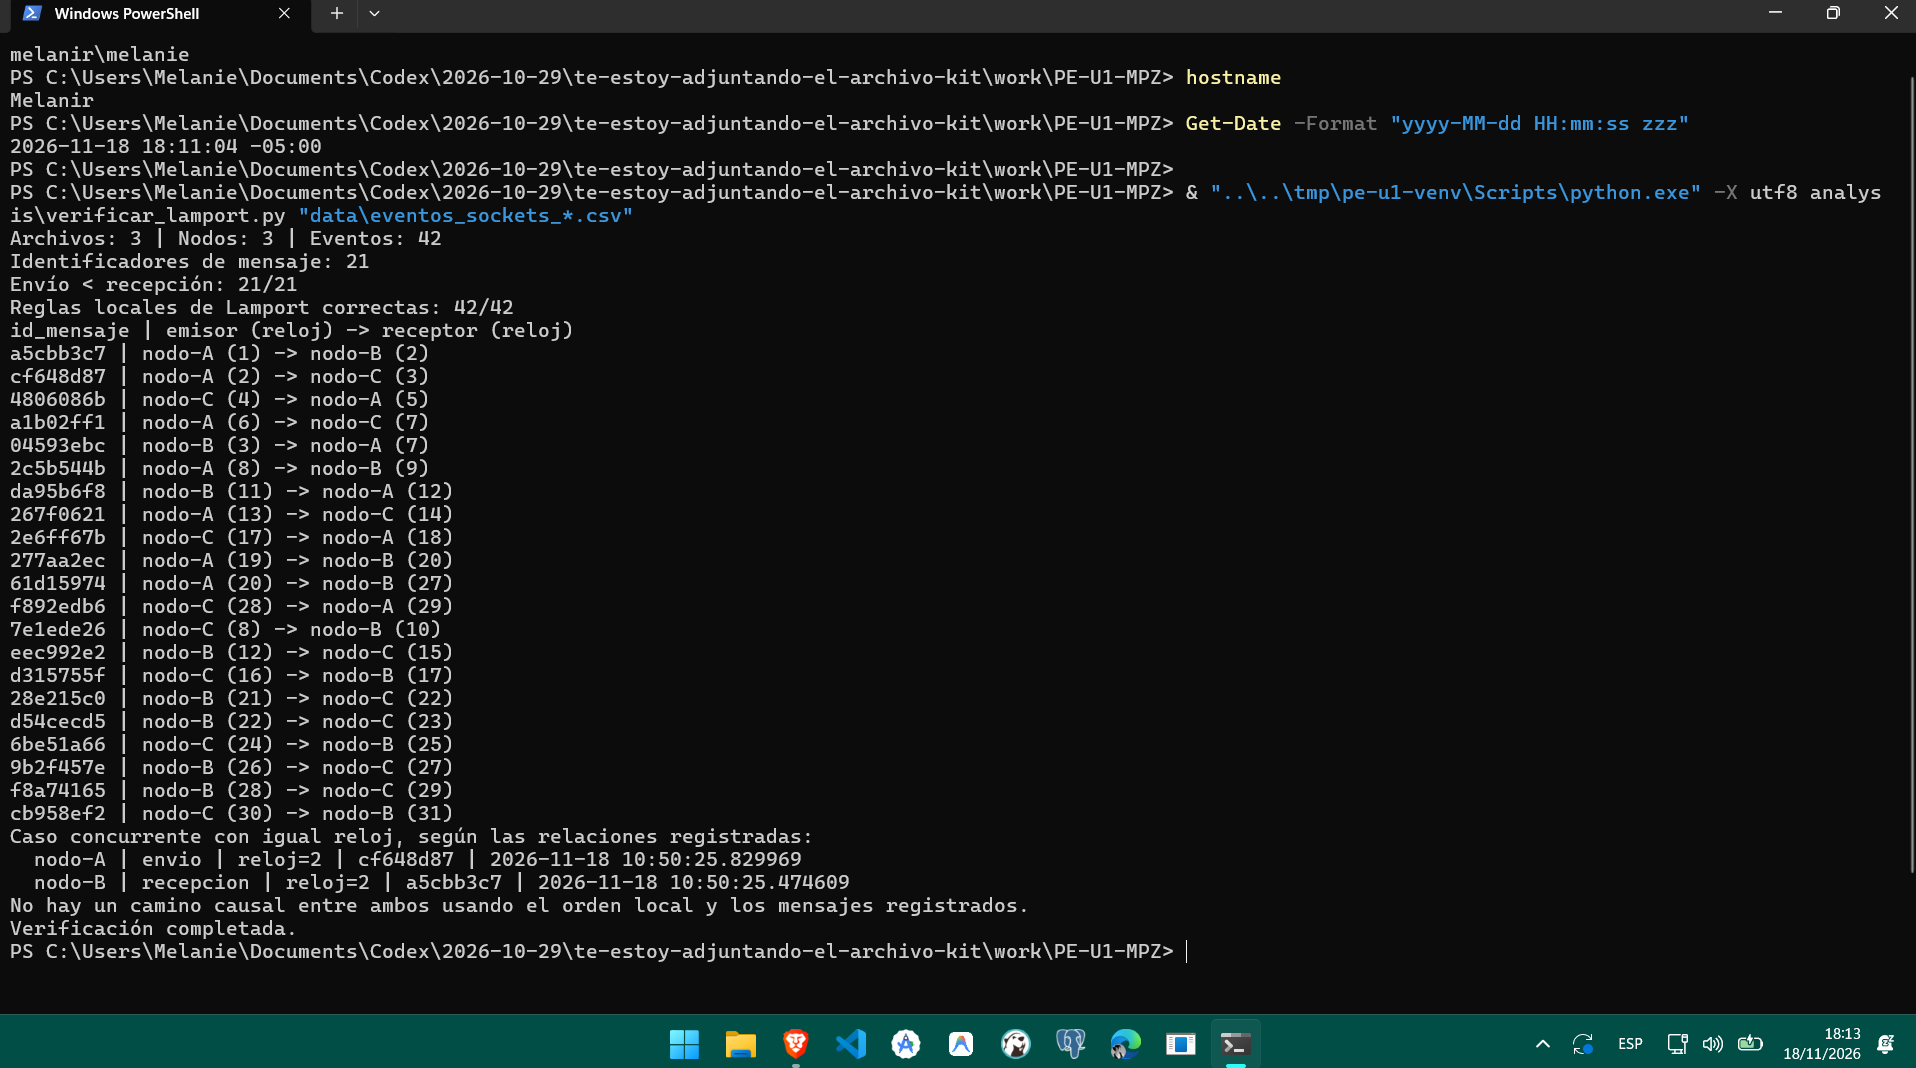
\includegraphics[width=\linewidth,height=0.72\textwidth,keepaspectratio]{../evidencias/melanie-verificacion-lamport.png}
\captionof{figure}{Ejecución del verificador de Lamport con los registros reales de sockets.}
\label{fig:lamport-melanie}
\end{center}
\end{landscape}
 desde docs/.
% Requiere amsmath, booktabs, graphicx, caption, pdflscape, hyperref y biblatex.
\section{Verificación del reloj de Lamport}
\label{sec:lamport}

\subsection{Procedimiento y resultados de sockets}
Se analizaron los tres archivos \texttt{eventos\_sockets\_nodo-*.csv}
de la carpeta \texttt{data/}, correspondientes a los nodos A, B y C
en la corrida de sockets del 18 de noviembre de 2026.

El programa \texttt{analysis/}\allowbreak\texttt{verificar\_lamport.py} empareja los eventos.
Se usa el campo \texttt{id\_mensaje} y se comprueba que las
contrapartes coincidan. Para las actualizaciones locales se conserva el
orden de las filas de cada nodo y se parte de un reloj igual a cero.

Antes de un envío, el valor esperado es $L_{\mathrm{nuevo}}=L_{\mathrm{local}}+1$.
Al recibir un mensaje, debe cumplirse
$L_{\mathrm{nuevo}}=\max(L_{\mathrm{local}},L_{\mathrm{enviado}})+1$.
También se comprueba que
$L_{\text{recepción}}>L_{\text{envío}}$ para cada mensaje.
Estas reglas siguen el tratamiento de relojes lógicos y orden causal
de van Steen y Tanenbaum \cite{vansteen2023distributed}.
La comprobación se ejecuta desde la raíz del repositorio:

\begin{quote}\small\ttfamily
python analysis/verificar\_lamport.py\par
\normalfont\small con el argumento \texttt{"data/eventos\_sockets\_*.csv"}.
\end{quote}

\begin{table}[htbp]
\centering
\caption{Resultados obtenidos con los registros reales de sockets.}
\label{tab:lamport-resultados}
\begin{tabular}{lr}
\toprule
\textbf{Comprobación} & \textbf{Resultado} \\
\midrule
Nodos registrados & 3 \\
Eventos registrados & 42 \\
Mensajes con envío y recepción emparejados & 21 \\
Mensajes con $L_{\text{recepción}}>L_{\text{envío}}$ & 21 de 21 \\
Eventos que cumplen la regla de actualización & 42 de 42 \\
\bottomrule
\end{tabular}
\end{table}

\subsection{Dos eventos concurrentes con el mismo reloj}
En esta corrida se encontró el par de la tabla~\ref{tab:lamport-concurrentes}.
El envío de \texttt{cf648d87} se dirige a nodo-C, mientras que la
recepción de \texttt{a5cbb3c7} corresponde a otro mensaje.
El verificador construye las relaciones de precedencia a partir del orden
local y de cada enlace envío--recepción. Al recorrerlas, no encuentra
un camino desde uno de estos eventos hasta el otro en ninguna dirección.

\begin{table}[htbp]
\centering
\caption{Ejemplo de concurrencia en los registros de sockets.}
\label{tab:lamport-concurrentes}
\small
\begin{tabular}{lllll}
\toprule
\textbf{Nodo} & \textbf{Evento} & \textbf{Mensaje} & \textbf{Reloj} & \textbf{Hora local} \\
\midrule
nodo-A & envio & \texttt{cf648d87} & 2 & 10:50:25.829969 \\
nodo-B & recepcion & \texttt{a5cbb3c7} & 2 & 10:50:25.474609 \\
\bottomrule
\end{tabular}
\end{table}

Ambos eventos tienen reloj 2. Esto muestra que los relojes de Lamport no
asignan un número único a cada evento. La propiedad de orden causal
establece que, si un evento precede causalmente a otro, su reloj es menor.
El recíproco no permite deducir causalidad: un valor menor tampoco
basta para afirmar que hubo influencia entre dos eventos.
Para este ejemplo, la concurrencia se contrasta con las relaciones de
los registros completos de la corrida. La diferencia entre las horas
físicas no establece por sí sola una relación causal
\cite{vansteen2023distributed}.

\begin{landscape}
\subsection{Evidencia de ejecución}
La figura~\ref{fig:lamport-melanie} muestra la ejecución del verificador
con los registros de sockets del grupo. La captura incluye el usuario,
el nombre de la máquina, la fecha, la hora del sistema y la salida completa.
\begin{center}
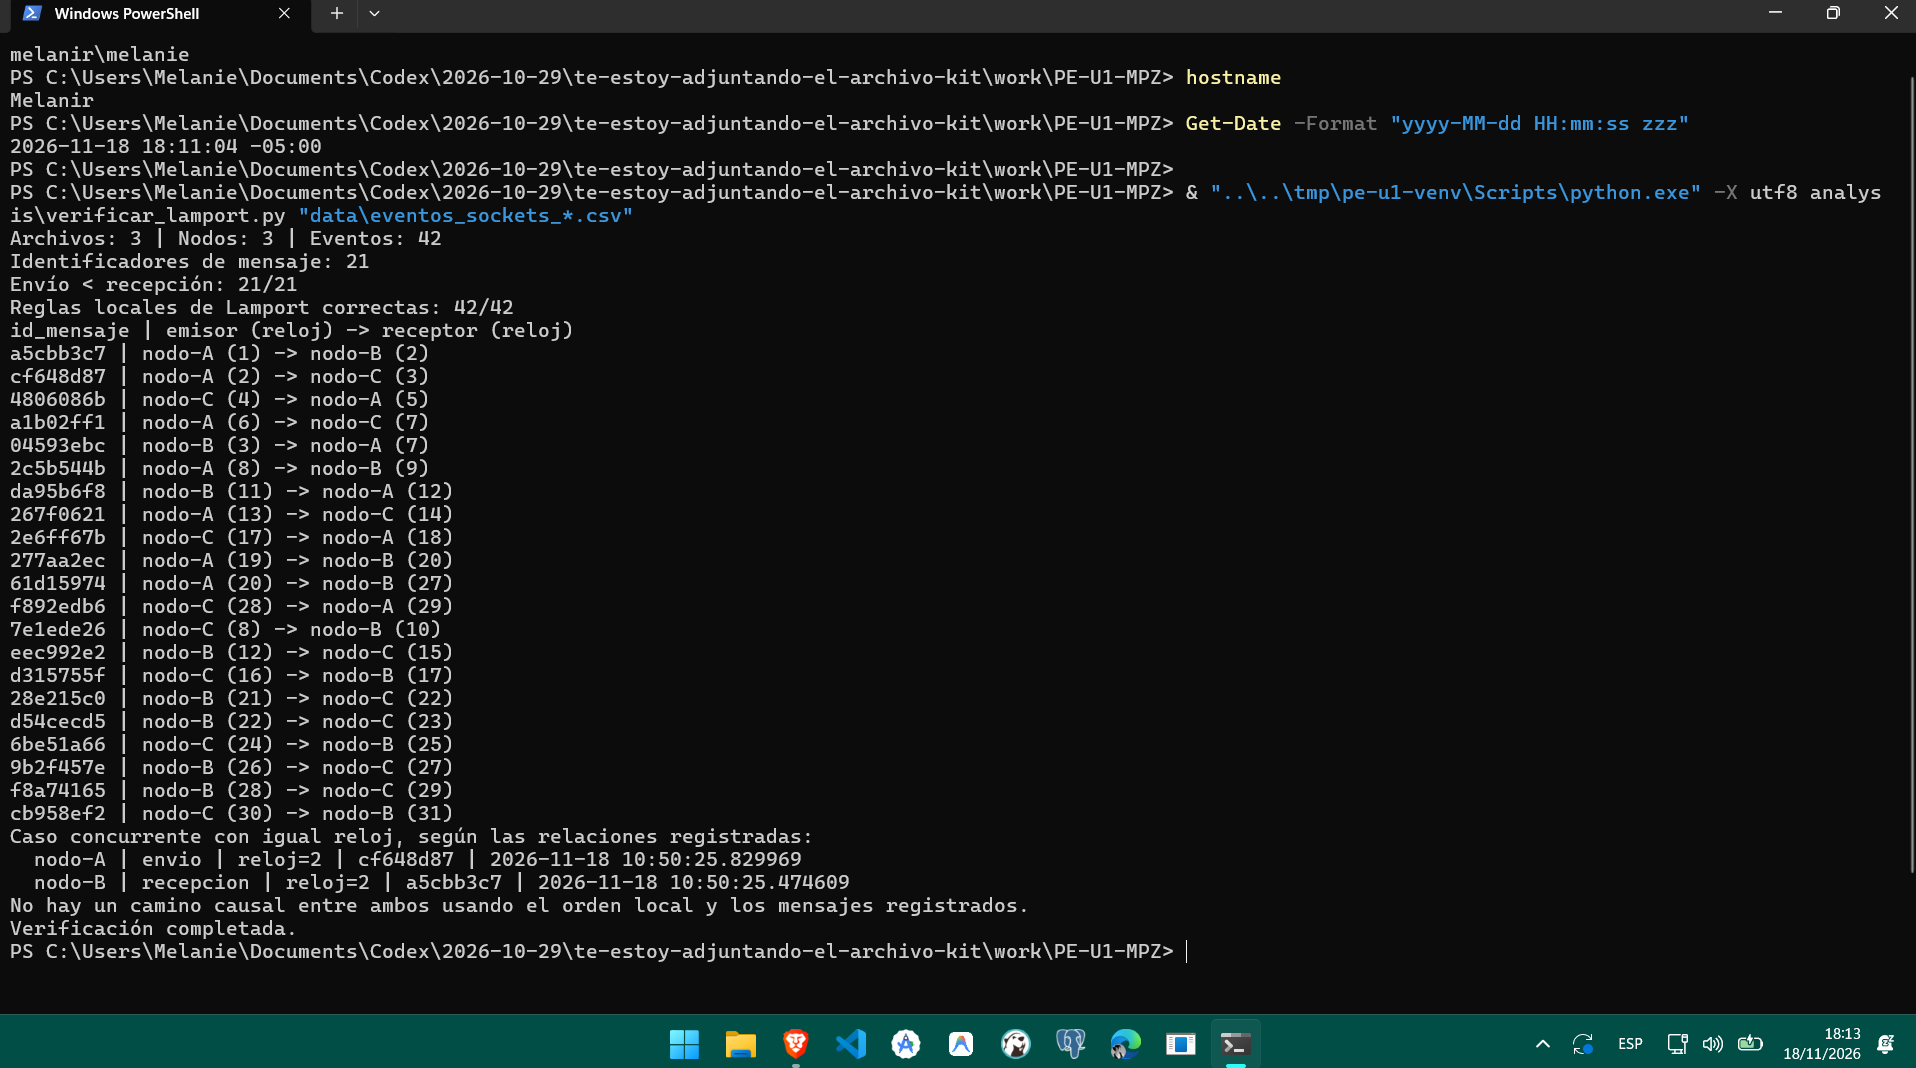
\includegraphics[width=\linewidth,height=0.72\textwidth,keepaspectratio]{../evidencias/melanie-verificacion-lamport.png}
\captionof{figure}{Ejecución del verificador de Lamport con los registros reales de sockets.}
\label{fig:lamport-melanie}
\end{center}
\end{landscape}
 desde docs/.
% Requiere amsmath, booktabs, graphicx, caption, pdflscape, hyperref y biblatex.
\section{Verificación del reloj de Lamport}
\label{sec:lamport}

\subsection{Procedimiento y resultados de sockets}
Se analizaron los tres archivos \texttt{eventos\_sockets\_nodo-*.csv}
de la carpeta \texttt{data/}, correspondientes a los nodos A, B y C
en la corrida de sockets del 18 de noviembre de 2026.

El programa \texttt{analysis/}\allowbreak\texttt{verificar\_lamport.py} empareja los eventos.
Se usa el campo \texttt{id\_mensaje} y se comprueba que las
contrapartes coincidan. Para las actualizaciones locales se conserva el
orden de las filas de cada nodo y se parte de un reloj igual a cero.

Antes de un envío, el valor esperado es $L_{\mathrm{nuevo}}=L_{\mathrm{local}}+1$.
Al recibir un mensaje, debe cumplirse
$L_{\mathrm{nuevo}}=\max(L_{\mathrm{local}},L_{\mathrm{enviado}})+1$.
También se comprueba que
$L_{\text{recepción}}>L_{\text{envío}}$ para cada mensaje.
Estas reglas siguen el tratamiento de relojes lógicos y orden causal
de van Steen y Tanenbaum \cite{vansteen2023distributed}.
La comprobación se ejecuta desde la raíz del repositorio:

\begin{quote}\small\ttfamily
python analysis/verificar\_lamport.py\par
\normalfont\small con el argumento \texttt{"data/eventos\_sockets\_*.csv"}.
\end{quote}

\begin{table}[htbp]
\centering
\caption{Resultados obtenidos con los registros reales de sockets.}
\label{tab:lamport-resultados}
\begin{tabular}{lr}
\toprule
\textbf{Comprobación} & \textbf{Resultado} \\
\midrule
Nodos registrados & 3 \\
Eventos registrados & 42 \\
Mensajes con envío y recepción emparejados & 21 \\
Mensajes con $L_{\text{recepción}}>L_{\text{envío}}$ & 21 de 21 \\
Eventos que cumplen la regla de actualización & 42 de 42 \\
\bottomrule
\end{tabular}
\end{table}

\subsection{Dos eventos concurrentes con el mismo reloj}
En esta corrida se encontró el par de la tabla~\ref{tab:lamport-concurrentes}.
El envío de \texttt{cf648d87} se dirige a nodo-C, mientras que la
recepción de \texttt{a5cbb3c7} corresponde a otro mensaje.
El verificador construye las relaciones de precedencia a partir del orden
local y de cada enlace envío--recepción. Al recorrerlas, no encuentra
un camino desde uno de estos eventos hasta el otro en ninguna dirección.

\begin{table}[htbp]
\centering
\caption{Ejemplo de concurrencia en los registros de sockets.}
\label{tab:lamport-concurrentes}
\small
\begin{tabular}{lllll}
\toprule
\textbf{Nodo} & \textbf{Evento} & \textbf{Mensaje} & \textbf{Reloj} & \textbf{Hora local} \\
\midrule
nodo-A & envio & \texttt{cf648d87} & 2 & 10:50:25.829969 \\
nodo-B & recepcion & \texttt{a5cbb3c7} & 2 & 10:50:25.474609 \\
\bottomrule
\end{tabular}
\end{table}

Ambos eventos tienen reloj 2. Esto muestra que los relojes de Lamport no
asignan un número único a cada evento. La propiedad de orden causal
establece que, si un evento precede causalmente a otro, su reloj es menor.
El recíproco no permite deducir causalidad: un valor menor tampoco
basta para afirmar que hubo influencia entre dos eventos.
Para este ejemplo, la concurrencia se contrasta con las relaciones de
los registros completos de la corrida. La diferencia entre las horas
físicas no establece por sí sola una relación causal
\cite{vansteen2023distributed}.

\begin{landscape}
\subsection{Evidencia de ejecución}
La figura~\ref{fig:lamport-melanie} muestra la ejecución del verificador
con los registros de sockets del grupo. La captura incluye el usuario,
el nombre de la máquina, la fecha, la hora del sistema y la salida completa.
\begin{center}
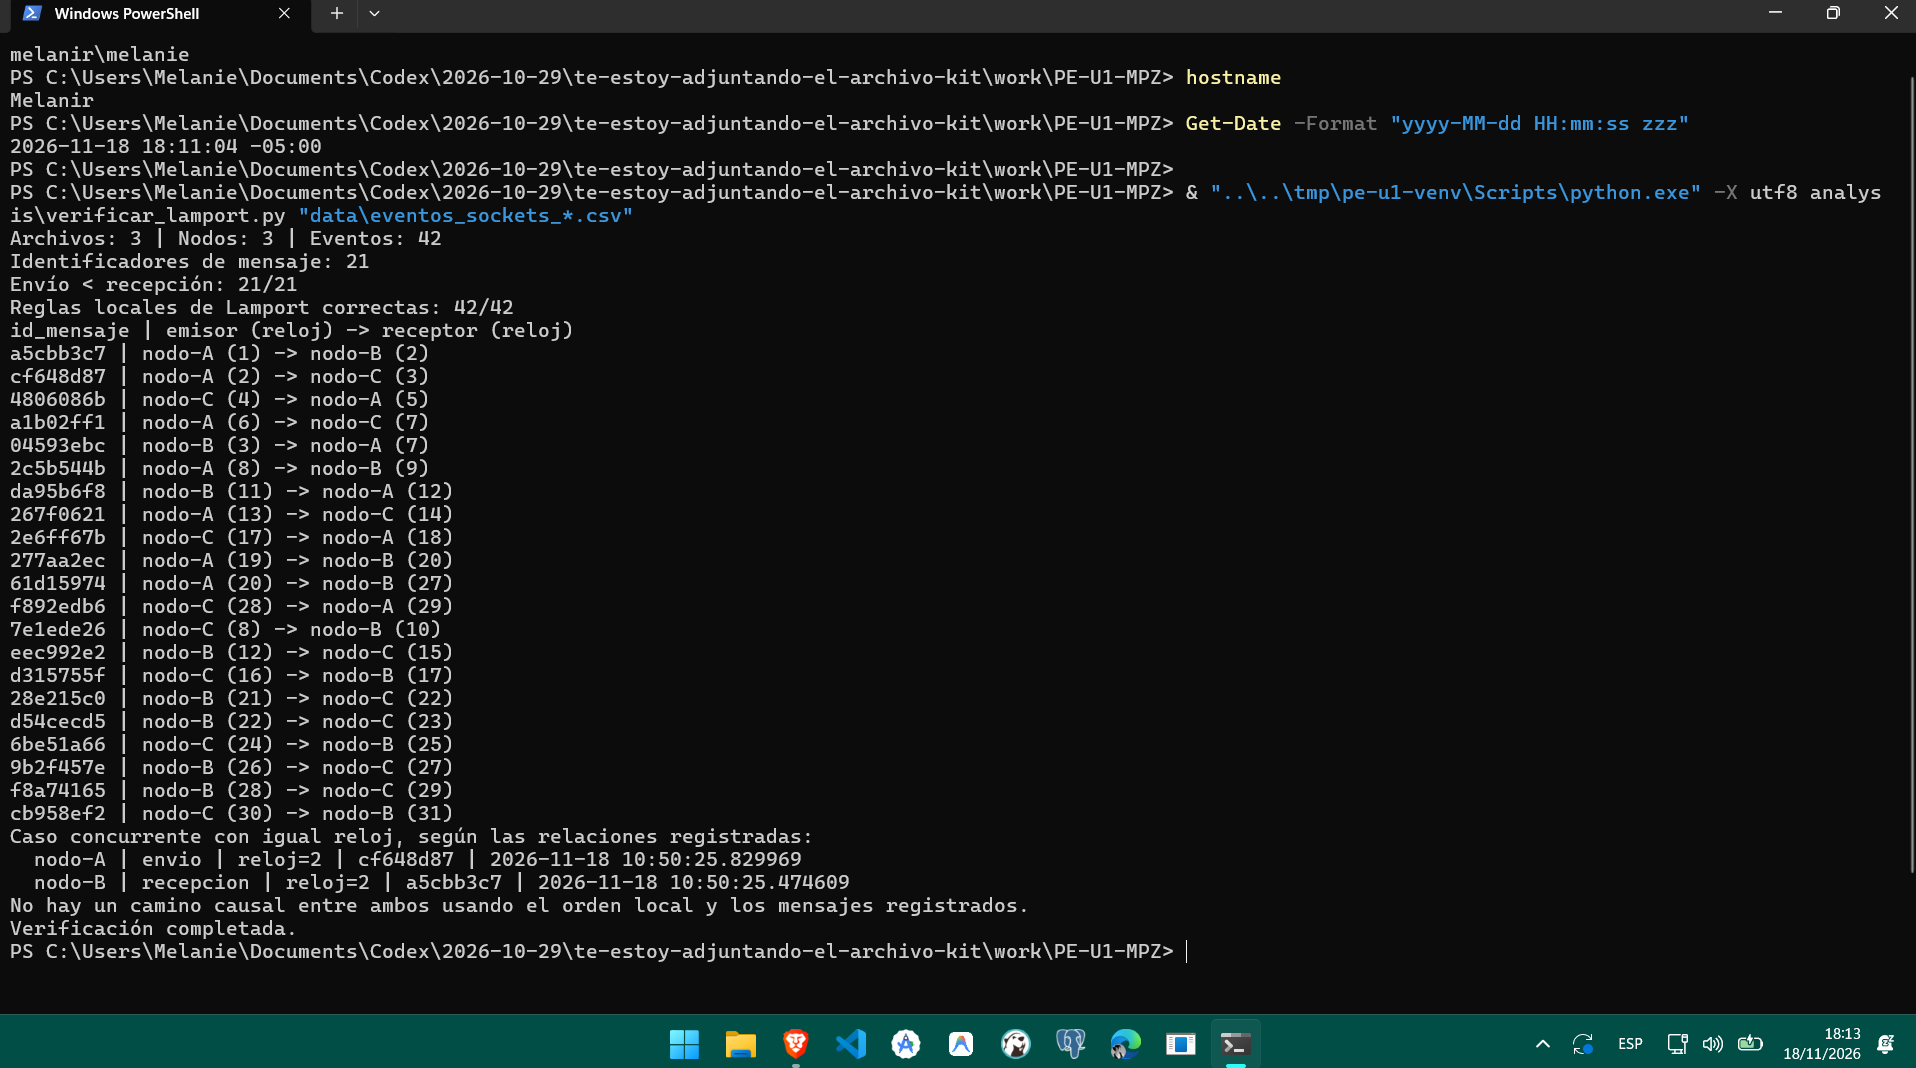
\includegraphics[width=\linewidth,height=0.72\textwidth,keepaspectratio]{../evidencias/melanie-verificacion-lamport.png}
\captionof{figure}{Ejecución del verificador de Lamport con los registros reales de sockets.}
\label{fig:lamport-melanie}
\end{center}
\end{landscape}

\printbibliography[title={Referencias}]
\end{document}
